\subsection{Gradient Ratio Results}
\label{subsection:gradienttresults}

\subsubsection{Regimes based on $R_\rho$ and $c$}
\label{subsubsection:gradientresultsR_Rhoandc}

The figure \ref{fig:gradient_results_r_rho_c_12} shows that for $c=1.2$ the regimes align with those found in \citet{McDougall1987}. These figures only extend to $R_\rho = \pm 13$ in order to better show the behaviour near the critical region $0<R_\rho<1$. There is a discontinuity at $R_\rho = 1.2$ as $R_\rho - c = 0$ at this point. In general the closer $R_\rho$ is to $c$ the smaller the denominator and hence the larger the overall gradient.   

We can see that there is a region $0<R_\rho<1$ in which the ratios of both $\theta$ and $S$ gradients are between 0 and 1, suggesting that the potential density surface is better aligned with the ``true" mixing direction. There is another region $R_\rho<0$ where the neutral surface has reduced $S$ gradients but increased $\theta$ gradients compared to a potential density surface. Finally there is the region $R_\rho>1$ where both gradients are larger on the potential density surface. This is as we theoretically predicted in section \ref{section:gradienttheorymathematical}.

\begin{figure}[htbp]
    \centering
    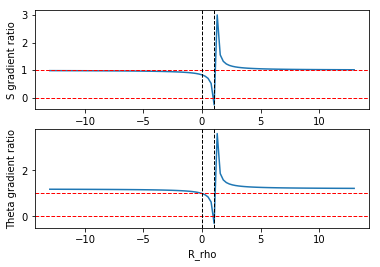
\includegraphics{gradient_regimes/R_rho_vs_gradient_12_e-1}
    \caption{The ratio of gradients of $S$ (top panel) and $\theta$ (bottom panel) against $R_\rho$ when $c=1.2$}
    \label{fig:gradient_results_r_rho_c_12}
\end{figure}

\begin{figure}[htbp]
    \centering
    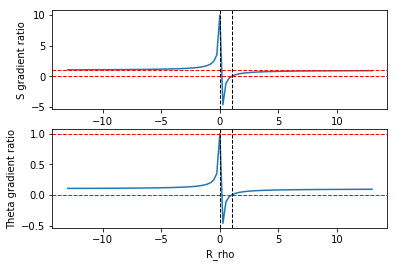
\includegraphics{gradient_regimes/R_rho_vs_gradient_1_e-1}
    \caption{The ratio of gradients of $S$ (top panel) and $\theta$ (bottom panel) against $R_\rho$ when $c=0.1$}
    \label{fig:gradient_results_r_rho_c_1}
\end{figure}

The second figure, \ref{fig:gradient_results_r_rho_c_1}, shows the gradient ratios of $\theta$ and $S$ when $c = 0.1$. As predicted, both the $\theta$ and $S$ gradients are reduced on the potential density surface compared to the neutral surface is in the region $R_\rho>1$.

Now we consider the full range of values of $R_\rho$ and $c$. The following figures only extend to $R_\rho = c = \pm 4$ in order to better show the behaviour near the critical region $0<R_\rho, c<1$. In figure \ref{fig:gradient_results_r_rho_vs_c_both_gradients} we can see the regions in which the gradient ratios are between 0 and 1. This is when the gradient on the potential density surface is smaller than on the neutral surface. If it is greater than 1 (dark grey) or less than 0 (light grey) then the neutral surface performs better.

\begin{figure}[htbp]
    \centering
    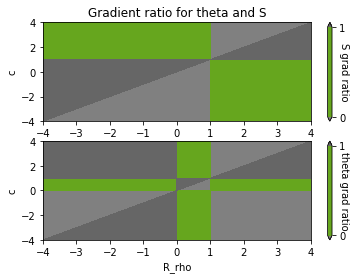
\includegraphics{gradient_regimes/R_rho_vs_c_s_and_theta_grad}
    \caption{The ratio of gradients of $S$(top panel) and $\theta$ (bottom panel) against $R_\rho$ and $c$}
    \label{fig:gradient_results_r_rho_vs_c_both_gradients}
\end{figure}

\begin{figure}[htbp]
    \centering
    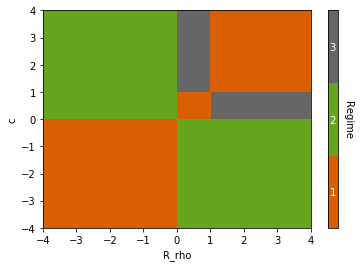
\includegraphics{gradient_regimes/regimes}
    \caption{Classification of regimes against $R_\rho$ and $c$. (1) Both $\theta$ and $S$ gradients are smallest on the neutral surface (2) $\theta$ or $S$ gradients are smallest on the neutral surface but not both, and (3) both $\theta$ and $S$ gradients are smallest on the potential density surface}
    \label{fig:gradient_results_regimes}
\end{figure}

The results for the $\theta$ and $S$ gradient ratios were then combined in figure \ref{fig:gradient_results_regimes} in order to classify the regimes which the ocean might be in. The final results are as follows:
\begin{enumerate}
    \item Both $\theta$ and $S$ gradients smallest on neutral surface
        \begin{itemize}
            \item $R_\rho>1$ and $c>1$ 
            \item $0<R_\rho<1$ and $0<c<1$
            \item $R_\rho<0$ and $c<0$
        \end{itemize}
    \item $\theta$ or $S$ gradients smaller on the neutral surface but not both
         \begin{itemize}
            \item $R_\rho<0$ and $c>0$
            \item $R_\rho>0$ and $c<0$
        \end{itemize}
    \item Both $\theta$ and $S$ gradients smallest on potential density surface
         \begin{itemize}
            \item $0<R_\rho<1$ and $c>1$
            \item $R_\rho>1$ and $0<c<1$
        \end{itemize}
\end{enumerate}

There are exceptions at $R_\rho = c$, where the gradient ratios cannot be defined, and at $R_\rho = 0$ or $c = 0$, where one or both of the gradient ratios are zero, which does not tell us anything meaningful. 

We can see that for $c<0$ we have either regime 1, where the neutral surface performs best, or regime 3 where neither the neutral surface or the potential density surface performs best for both $\theta$ and $S$. 

For $c>0$ the results are as we predicted in section \ref{subsection:gradienttheorymathematicaltheory}. For $R_\rho<0$ we are in regime 3, where neither surface performs better for both variables. For $R_\rho>0$ we can find a potential density surface that has reduced gradients for both $\theta$ and $S$ either in the region $0<c<1$ or $c>1$ depending on the value of $R_\rho$. 

It is interesting that each regime does not correspond simply to the classifications of the density ratio; if we have $R_\rho>1$, where ``salt fingering" is possible, it is not guaranteed that we will be in regime 1, for example. The value of $c$ is important in determining which regime we will be in. 

\subsubsection{Atlantic}
\label{subsubsection:gradientresultsAtlantic}

In \citet{McDougall1987} the variables $S$ and $\theta$ are shown projected onto various $\sigma$ and $\gamma_n$ surfaces in order to visually quantify the gradient. This paper replicates those figures, presented in section \ref{section:spread} and appendix \ref{appendix_a}, but those results should be predictable from the mathematical theory. 

To that end, real ocean data from the \citet{WOCE2002} dataset was used in order to calculate $R_\rho$, $c$ and the two gradient ratios for $R_\rho$ and $S$. This also allows the region to be categorised into the regimes outlined in the previous subsection. 

At the location of the surfaces of interest given in \ref{subsection:spreadmethod},  $5^{\circ}$N and $47^{\circ}$W at a depth of 1750m, the value of $R_\rho$ was calculated to be 16.7 (3 s.f.). The values of $c$ at the reference pressures 0dbar, 2000dbar and 4000dbar were as follows:

\begin{itemize}
    \item $c_{\sigma_0} = 1.48$
    \item $c_{\sigma_2} = 0.96$
    \item $c_{\sigma_4} = 0.72$
\end{itemize}

This places the starting point for the surfaces in regime 3, as given in the previous subsection. Hence we might expect that the gradient ratios of both $S$ and $\theta$ will be between 0 and 1 on the $\sigma_2$ and $\sigma_4$ surfaces.

\begin{figure}[htbp]
    \centering
     
     \begin{subfigure}{0.4\textwidth}
         
         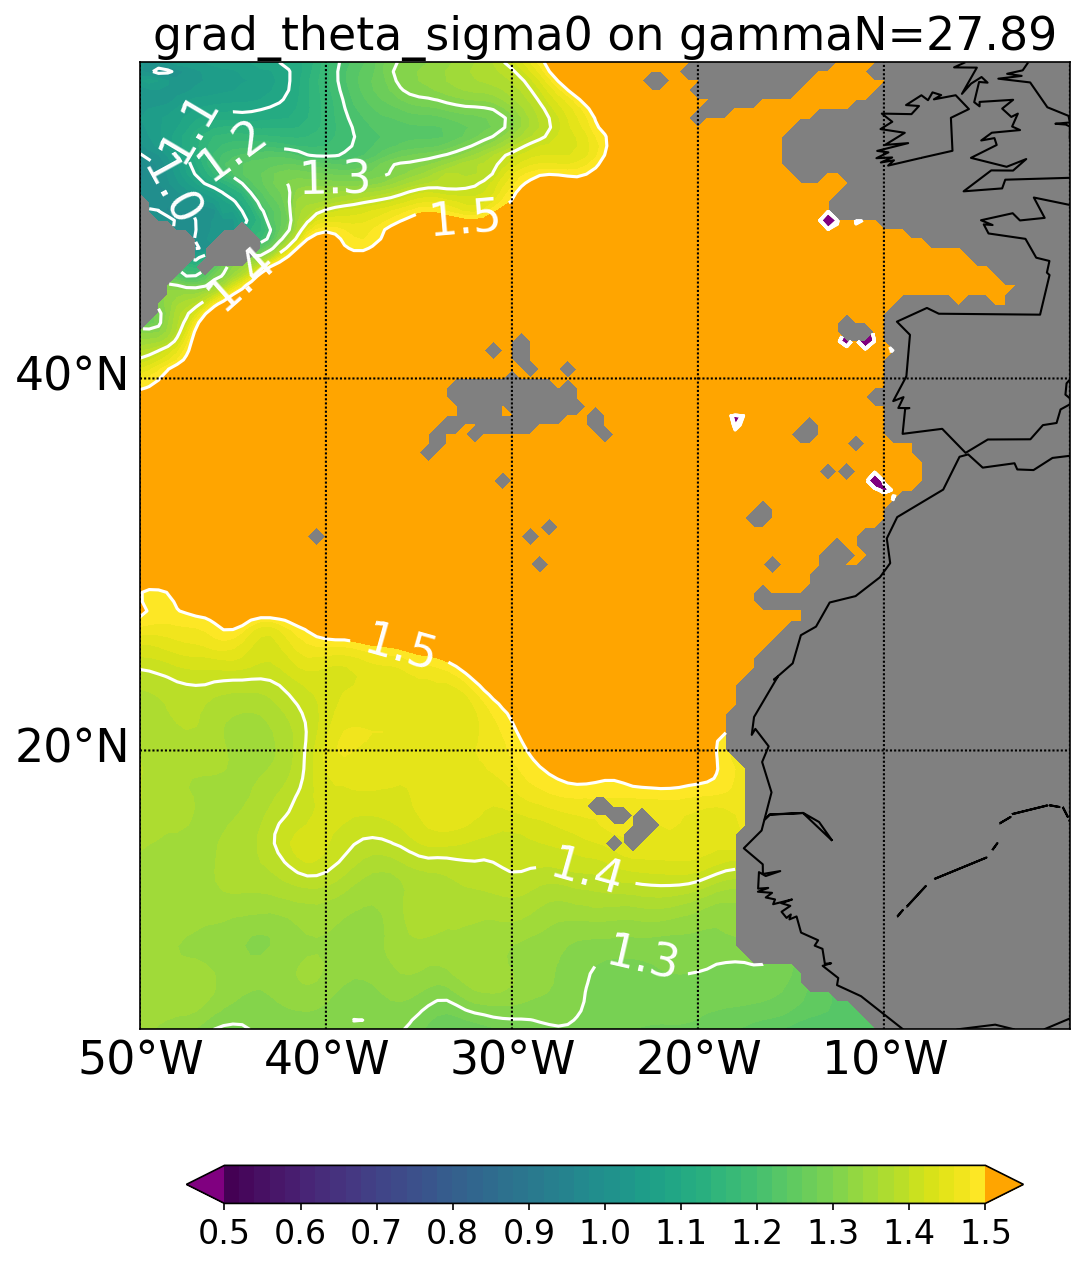
\includegraphics[width=\textwidth]{gradient_ratios/atlantic_grad_theta/Map2dcyl_grad_theta_sigma0_on_gammaN_2789e-2_reg310Eto360E05Nto57N_1990to1998av_WOCE}
         \caption{Referenced to $p_{ref} = 0$dbar}
         \label{fig:subplot_atlantic_grad_theta_sig0}
     \end{subfigure}
     \begin{subfigure}{0.4\textwidth}
         
         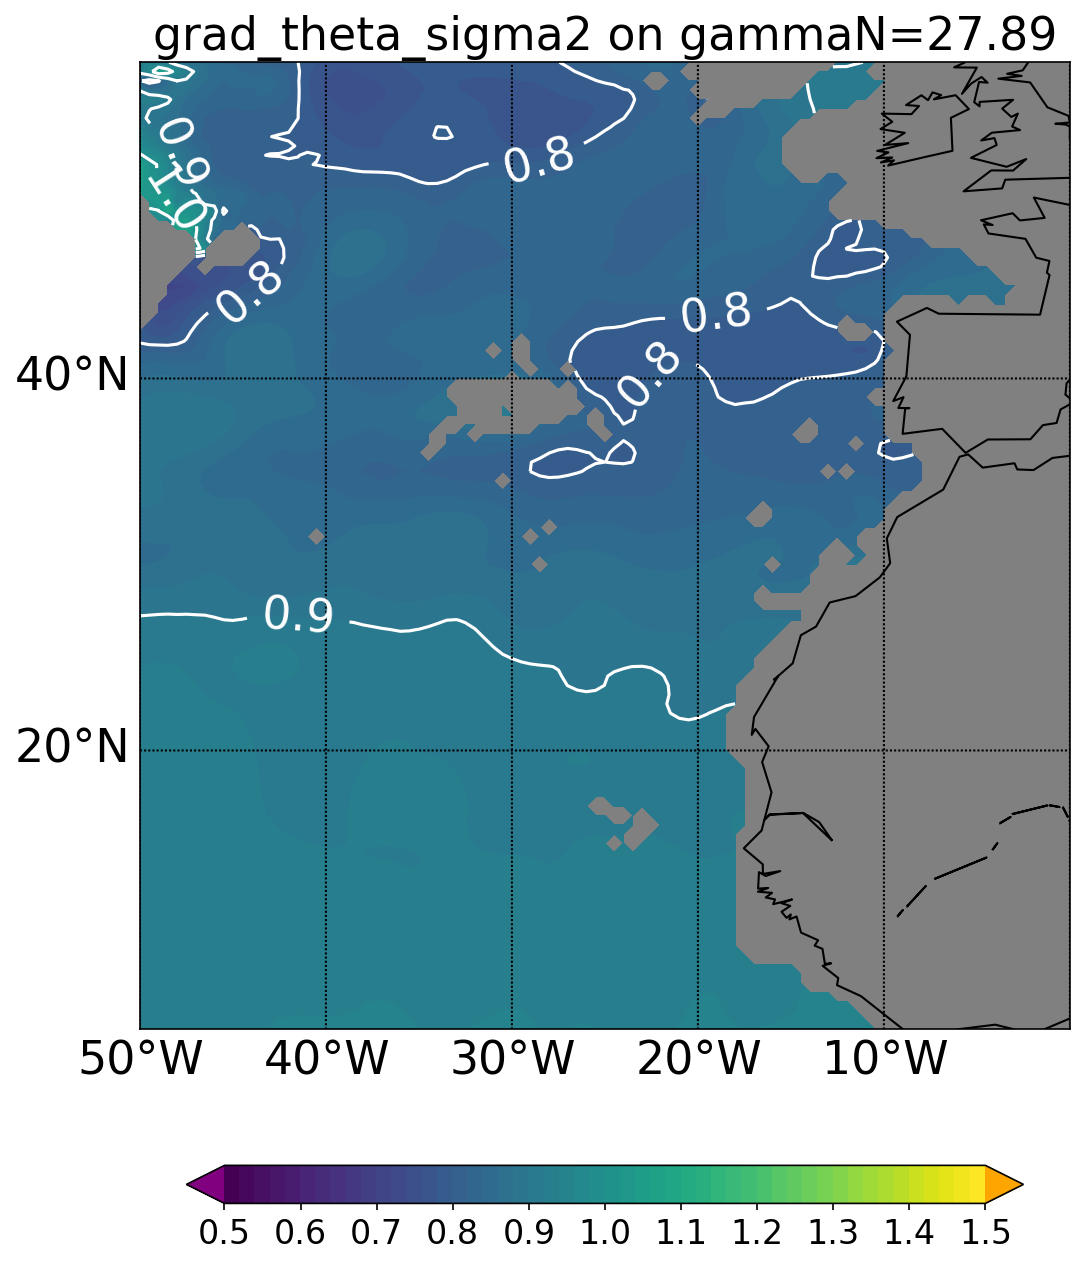
\includegraphics[width=\textwidth]{gradient_ratios/atlantic_grad_theta/Map2dcyl_grad_theta_sigma2_on_gammaN_2789e-2_reg310Eto360E05Nto57N_1990to1998av_WOCE}
         \caption{Referenced to $p_{ref} = 2000$dbar}
         \label{fig:subplot_atlantic_grad_theta_sig2}
     \end{subfigure}
     
     \begin{subfigure}{0.4\textwidth}
         
         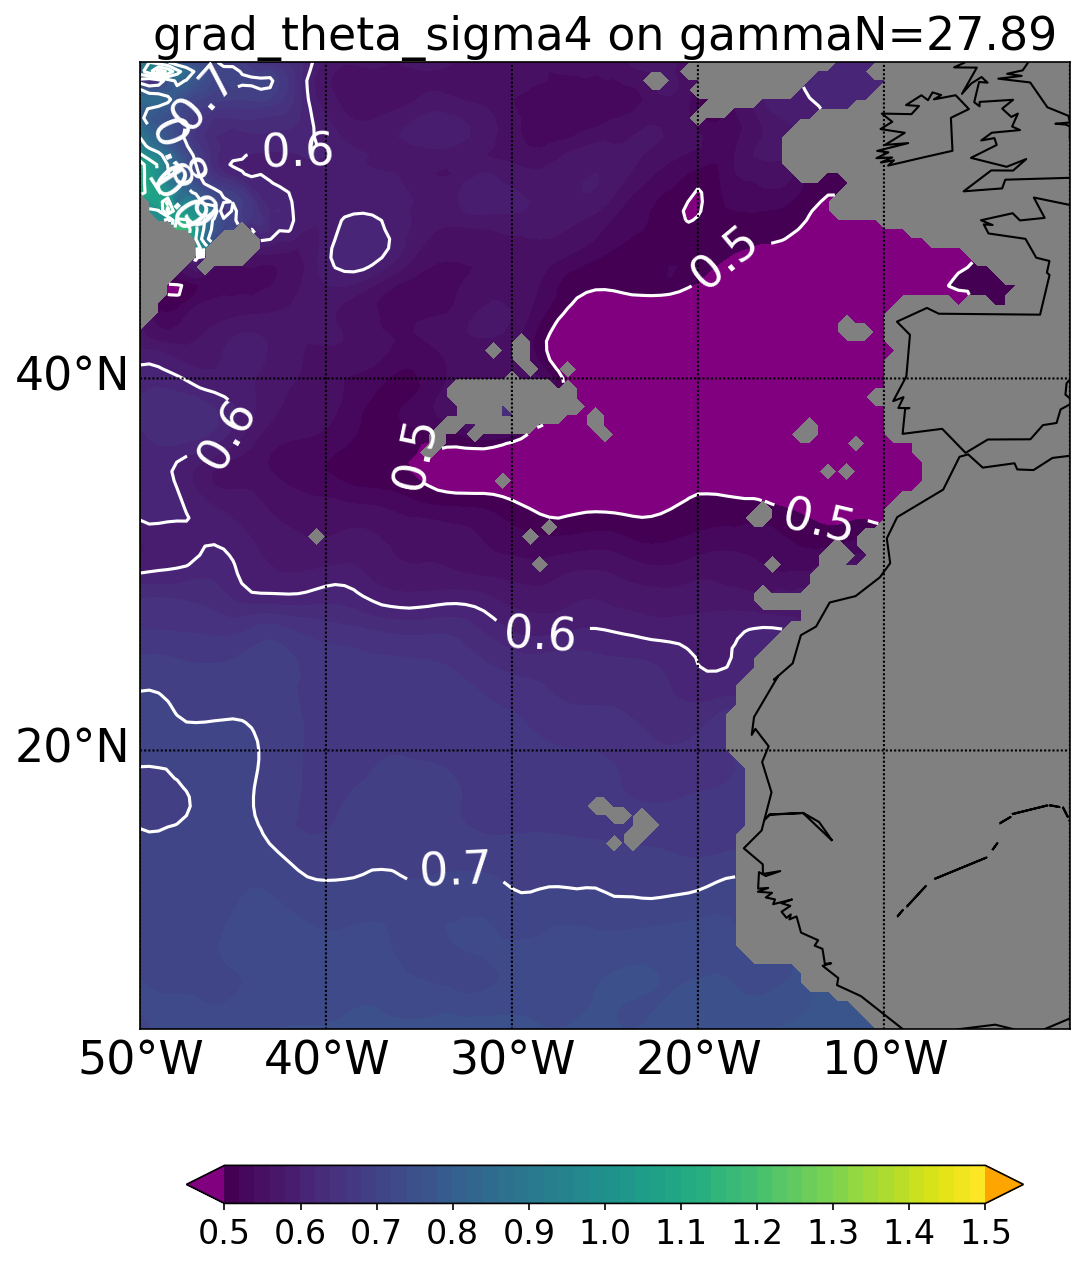
\includegraphics[width=\textwidth]{gradient_ratios/atlantic_grad_theta/Map2dcyl_grad_theta_sigma4_on_gammaN_2789e-2_reg310Eto360E05Nto57N_1990to1998av_WOCE}
         \caption{$\sigma_4$ where $p_{ref} = 4000$dbar}
         \label{fig:subplot_atlantic_grad_theta_sig4}
     \end{subfigure}
    \caption{Gradient ratio of $\theta$ for three reference pressures, 0, 2000 and 4000dbar which correspond to the $\sigma_0$, $\sigma_2$ and $\sigma_4$ potential density surfaces respectively, projected onto the neutral surface $\gamma_n = 27.89$, Atlantic region (see section \ref{subsubsection:spreadmethodatlanticocean})}
    \label{fig:atlantic_grad_theta}
    
\end{figure}


\begin{figure}[htbp]
    \centering
     
     \begin{subfigure}{0.4\textwidth}
         
         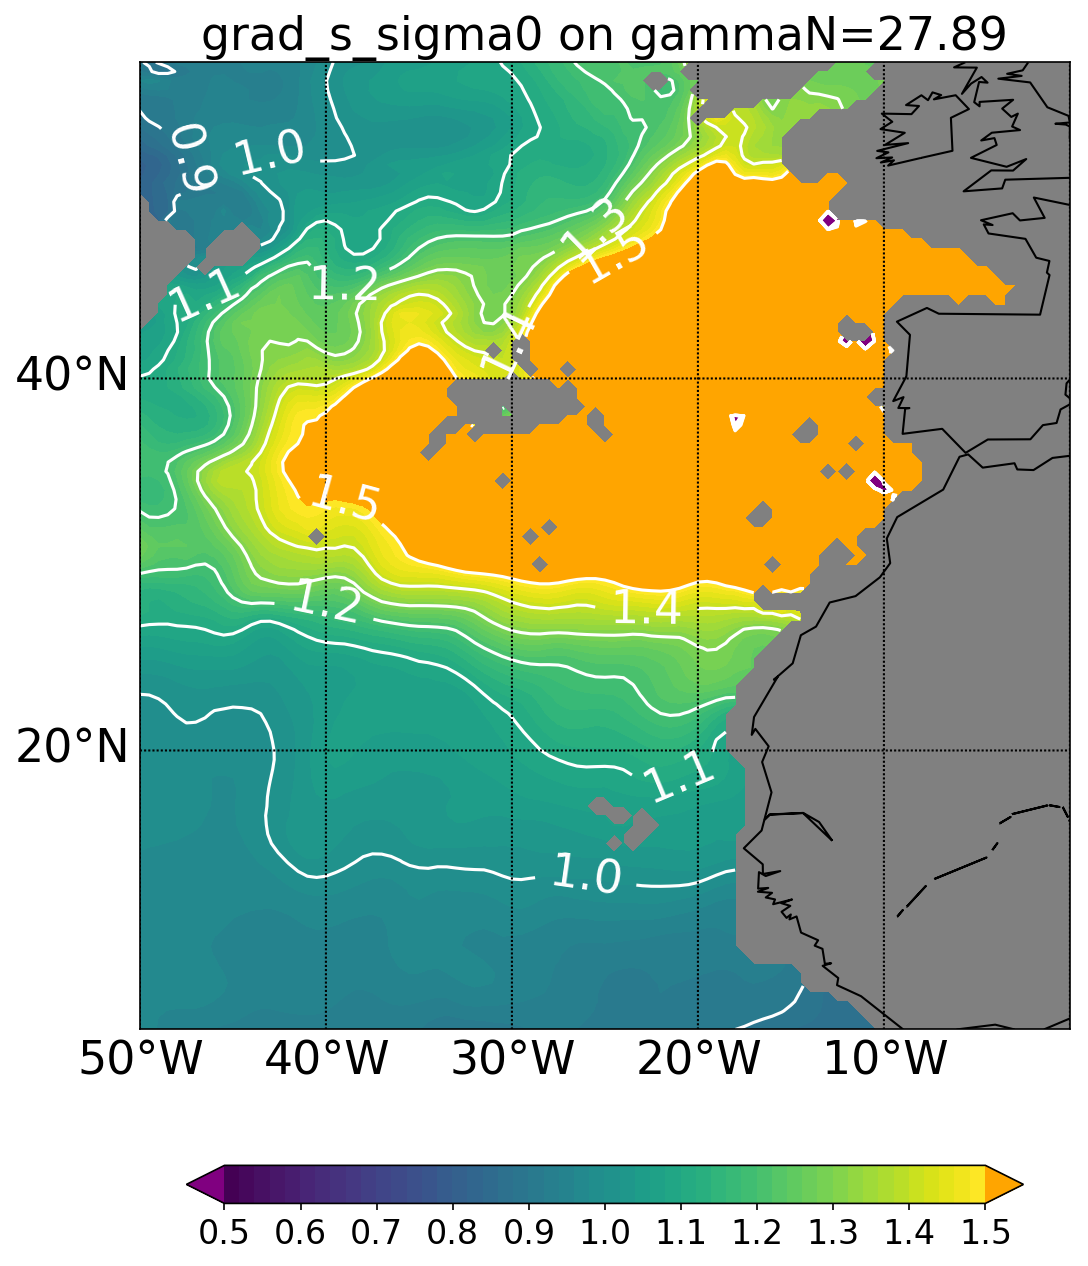
\includegraphics[width=\textwidth]{gradient_ratios/atlantic_grad_s/Map2dcyl_grad_s_sigma0_on_gammaN_2789e-2_reg310Eto360E05Nto57N_1990to1998av_WOCE}
         \caption{Referenced to $p_{ref} = 0$dbar}
         \label{fig:subplot_atlantic_grad_s_sig0}
     \end{subfigure}
     \begin{subfigure}{0.4\textwidth}
         
         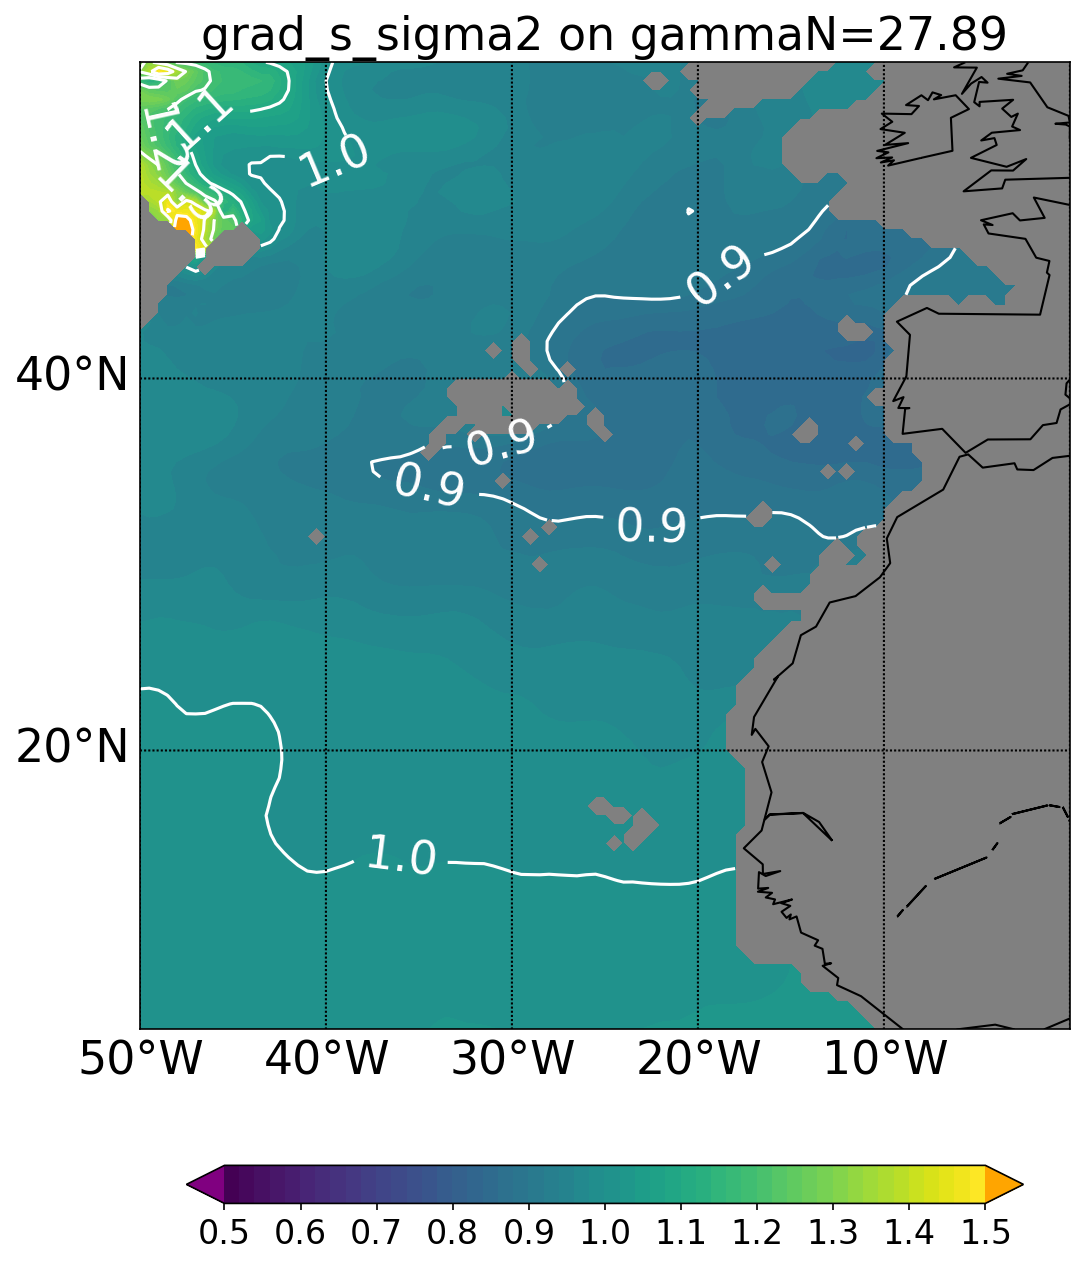
\includegraphics[width=\textwidth]{gradient_ratios/atlantic_grad_s/Map2dcyl_grad_s_sigma2_on_gammaN_2789e-2_reg310Eto360E05Nto57N_1990to1998av_WOCE}
         \caption{Referenced to $p_{ref} = 2000$dbar}
         \label{fig:subplot_atlantic_grad_s_sig2}
     \end{subfigure}
     
     \begin{subfigure}{0.4\textwidth}
         
         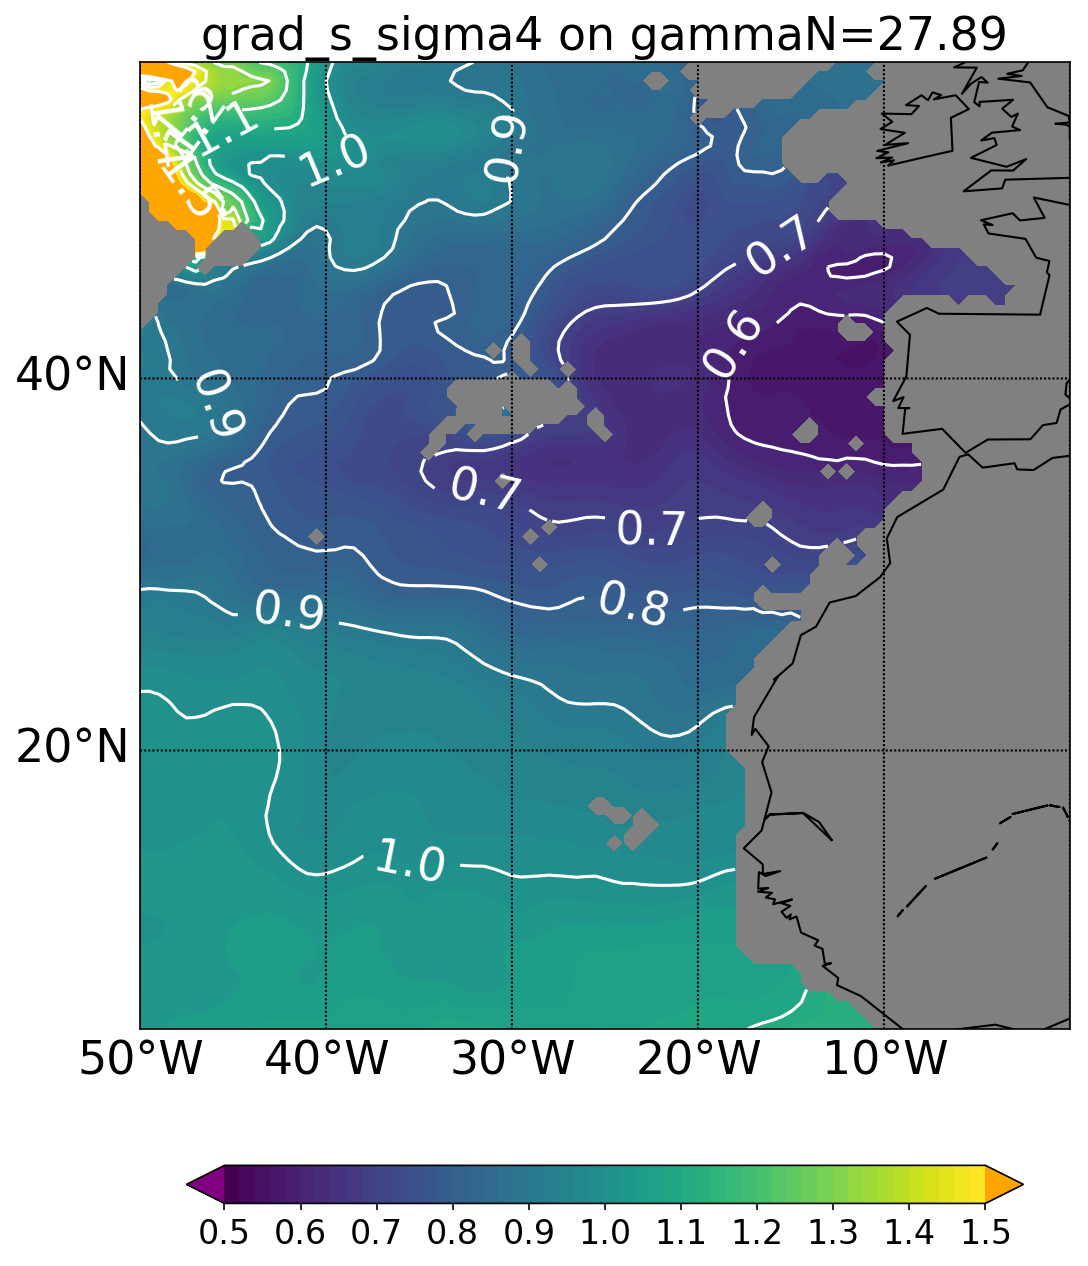
\includegraphics[width=\textwidth]{gradient_ratios/atlantic_grad_s/Map2dcyl_grad_s_sigma4_on_gammaN_2789e-2_reg310Eto360E05Nto57N_1990to1998av_WOCE}
         \caption{$\sigma_4$ where $p_{ref} = 4000$dbar}
         \label{fig:subplot_atlantic_grad_s_sig4}
     \end{subfigure}
    \caption{Gradient ratio of $S$ for three reference pressures, 0, 2000 and 4000dbar which correspond to the $\sigma_0$, $\sigma_2$ and $\sigma_4$ potential density surfaces respectively, projected onto the neutral surface $\gamma_n = 27.89$, Atlantic region (see section \ref{subsubsection:spreadmethodatlanticocean})}
    \label{fig:atlantic_grad_s}
    
\end{figure}

We can clearly see from figures \ref{fig:atlantic_grad_theta} and \ref{fig:atlantic_grad_s} that we should expect reduced ``spread" of both $\theta$ and $S$ on the $\sigma_2$ and $\sigma_4$ surfaces when compared to the $\gamma_n$ surface as the gradient ratios are between 0 and 1, as predicted by the values of $R_\rho$ and $c$. The surface $\sigma_0$ has both gradient ratios larger than 1, so we predict that the ``spread" of $\theta$ and $S$ on this surface will be larger than on the $\gamma_n$ surface. 

\subsubsection{Gibraltar Straight}
\label{subsubseciton:gradientresultsGibraltar}

The value of $R_\rho$ at the location at which the surfaces of interest were calculated, $36^{\circ}$N and $8^{\circ}$W at a depth of 1200m, was -7.40 (rounded to 3 s.f.). The values of $c$ referenced to the three reference depths were 

\begin{itemize}
    \item $c_{\sigma_0} = 1.15$
    \item $c_{\sigma_2} = 0.92$
    \item $c_{\sigma_4} = 0.77$
\end{itemize}

This puts the starting point in regime 2, where the gradients are smaller on the neutral surface for $\theta$ or $c$ but not both.

\begin{figure}[htbp]
    \centering
     
     \begin{subfigure}{0.4\textwidth}
         
         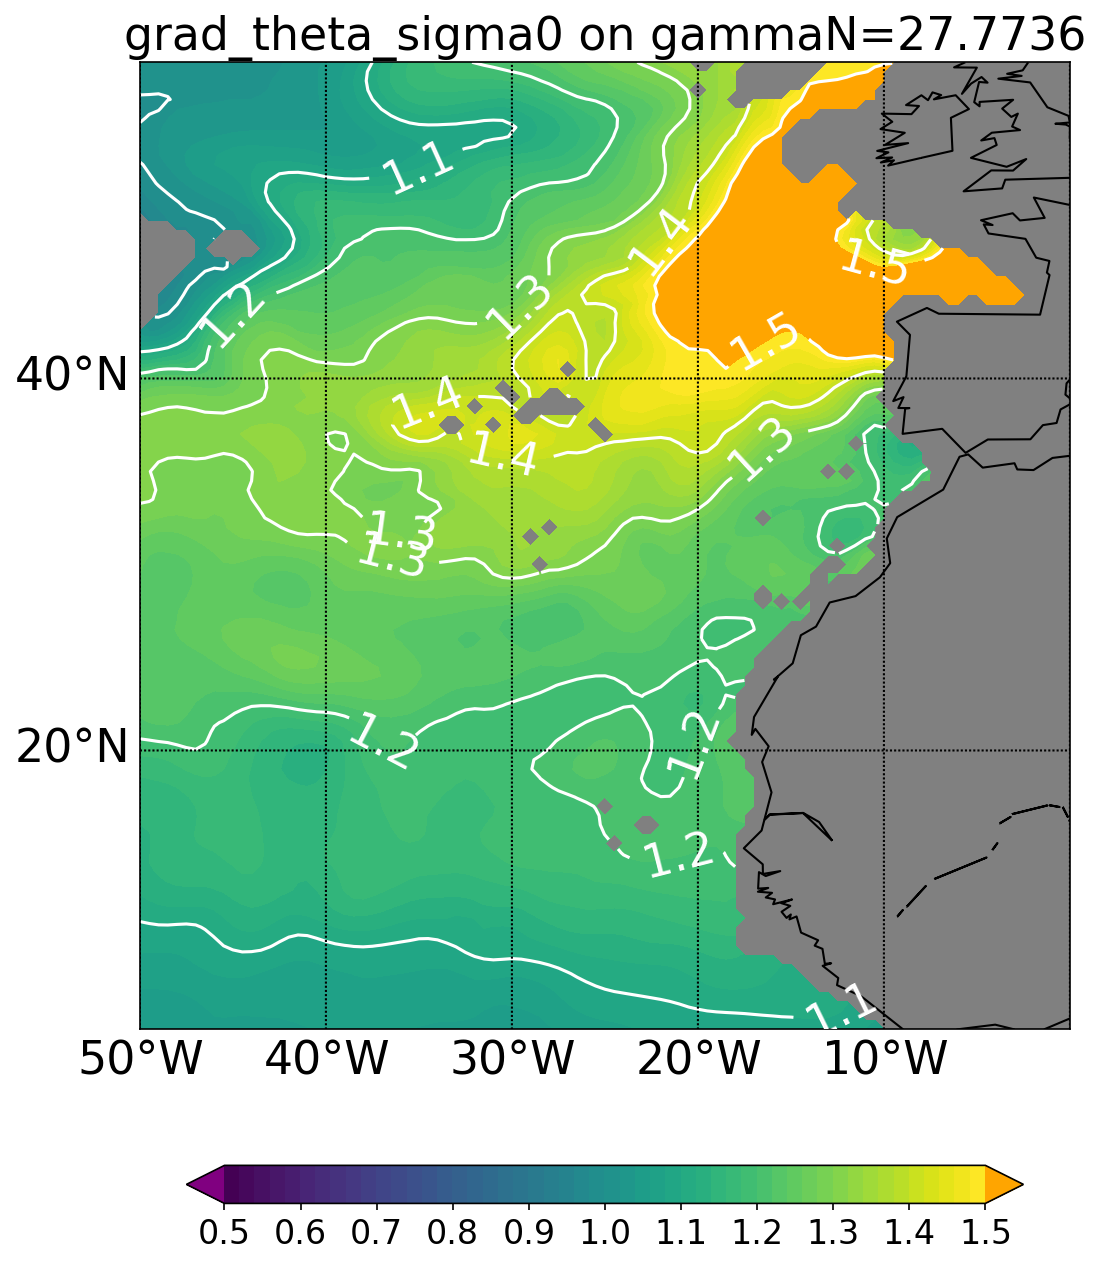
\includegraphics[width=\textwidth]{gradient_ratios/gibraltar_grad_theta/Map2dcyl_grad_theta_sigma0_on_gammaN_2777e-2_reg310Eto360E05Nto57N_1990to1998av_WOCE}
         \caption{Referenced to $p_{ref} = 0$dbar}
         \label{fig:subplot_gibraltar_grad_theta_sig0}
     \end{subfigure}
     \begin{subfigure}{0.4\textwidth}
         
         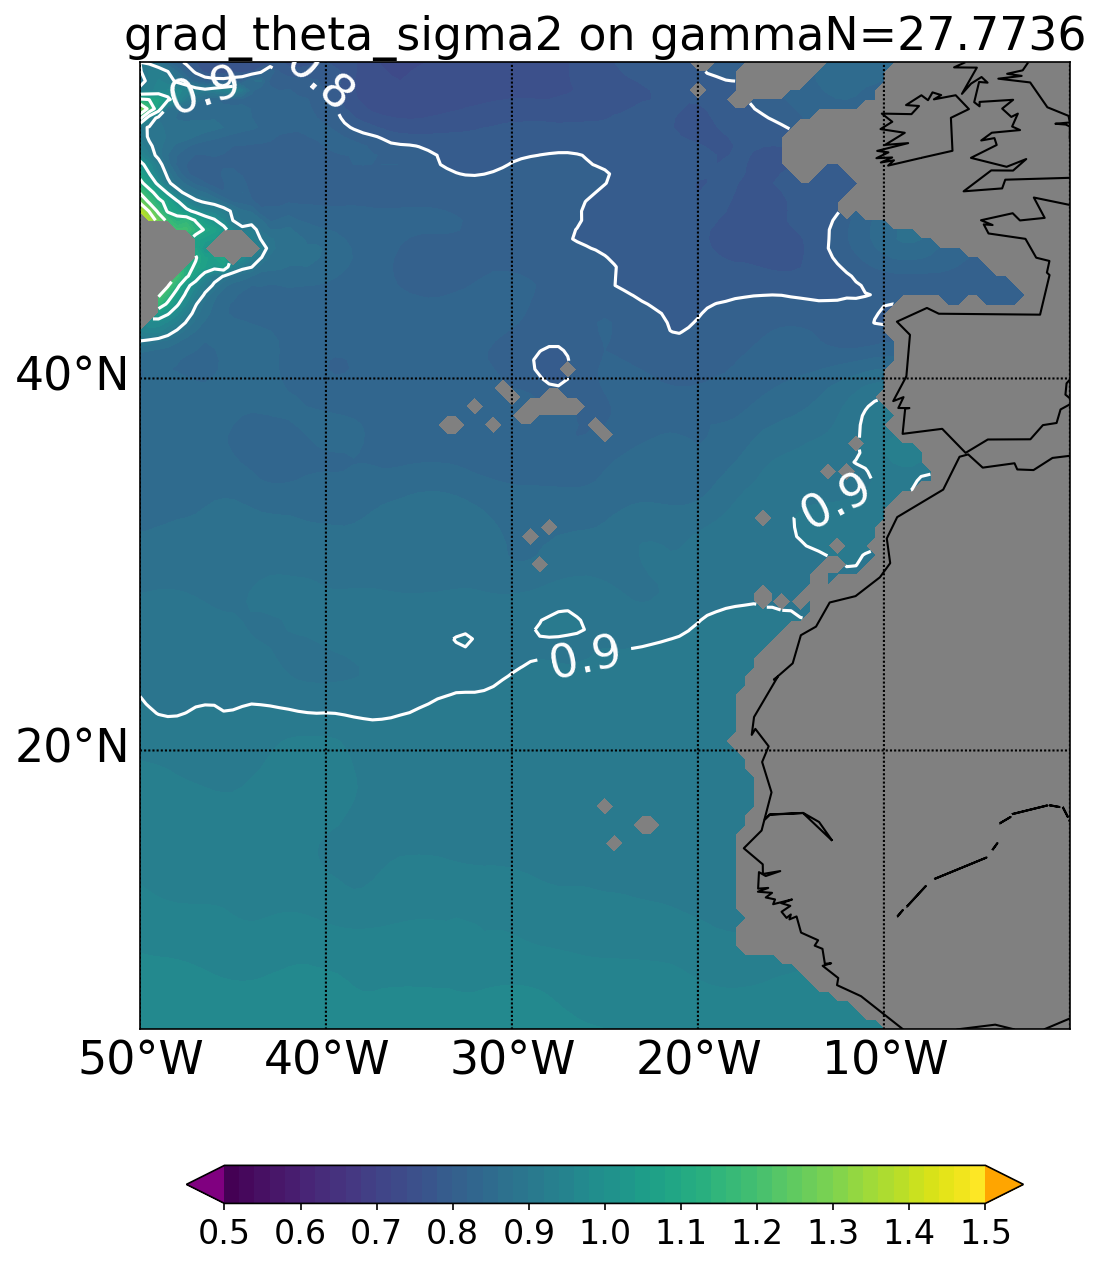
\includegraphics[width=\textwidth]{gradient_ratios/gibraltar_grad_theta/Map2dcyl_grad_theta_sigma2_on_gammaN_2777e-2_reg310Eto360E05Nto57N_1990to1998av_WOCE}
         \caption{Referenced to $p_{ref} = 2000$dbar}
         \label{fig:subplot_gibraltar_grad_theta_sig2}
     \end{subfigure}
     
     \begin{subfigure}{0.4\textwidth}
         
         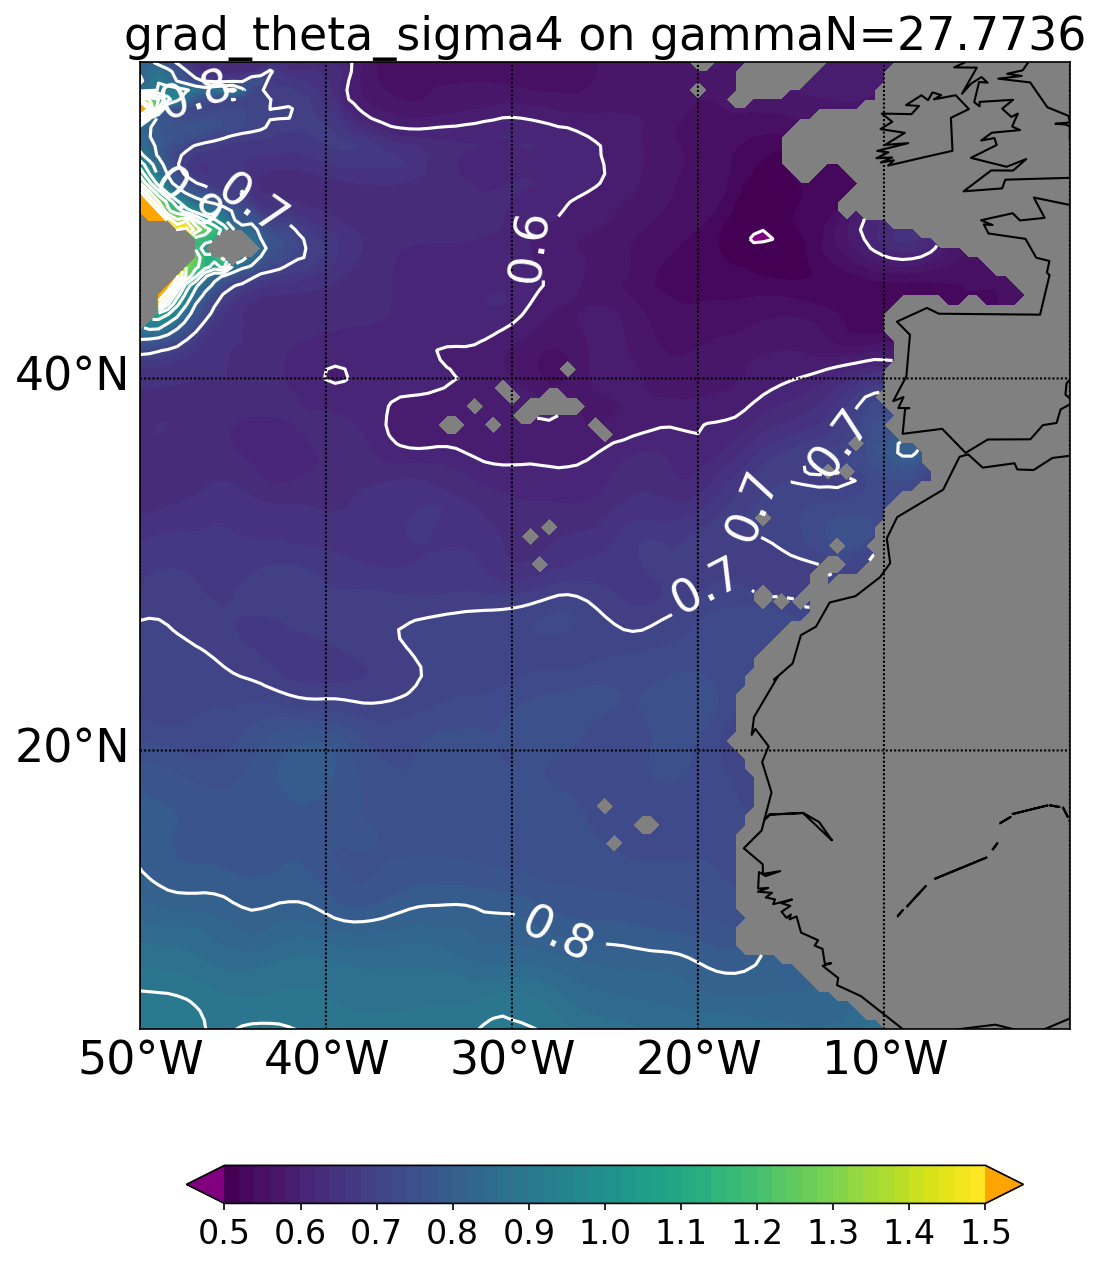
\includegraphics[width=\textwidth]{gradient_ratios/gibraltar_grad_theta/Map2dcyl_grad_theta_sigma4_on_gammaN_2777e-2_reg310Eto360E05Nto57N_1990to1998av_WOCE}
         \caption{$\sigma_4$ where $p_{ref} = 4000$dbar}
         \label{fig:subplot_gibraltar_grad_theta_sig4}
     \end{subfigure}
    \caption{Gradient ratio of $\theta$ for three reference pressures, 0, 2000 and 4000dbar which correspond to the $\sigma_0$, $\sigma_2$ and $\sigma_4$ potential density surfaces respectively, projected onto the neutral surface $\gamma_n = 27.7736$, Gibraltar Region (see section \ref{subsubsection:spreadmethodgibraltarstraight})}
    \label{fig:gibraltar_grad_theta}
    
\end{figure}


\begin{figure}[htbp]
    \centering
     
     \begin{subfigure}{0.4\textwidth}
         
         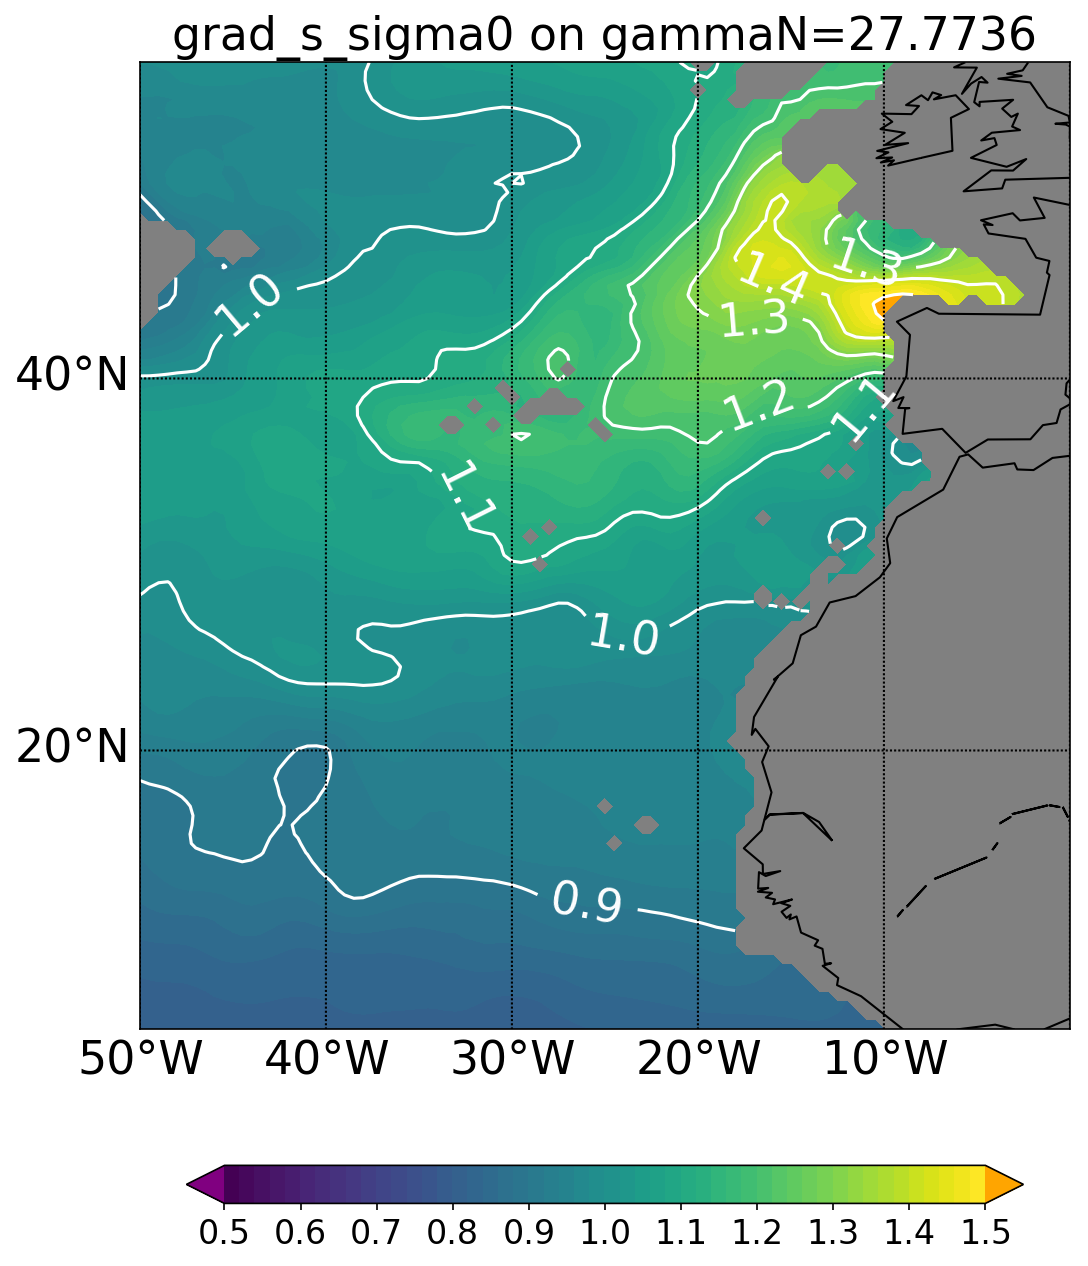
\includegraphics[width=\textwidth]{gradient_ratios/gibraltar_grad_s/Map2dcyl_grad_s_sigma0_on_gammaN_2777e-2_reg310Eto360E05Nto57N_1990to1998av_WOCE}
         \caption{Referenced to $p_{ref} = 0$dbar}
         \label{fig:subplot_gibraltar_grad_s_sig0}
     \end{subfigure}
     \begin{subfigure}{0.4\textwidth}
         
         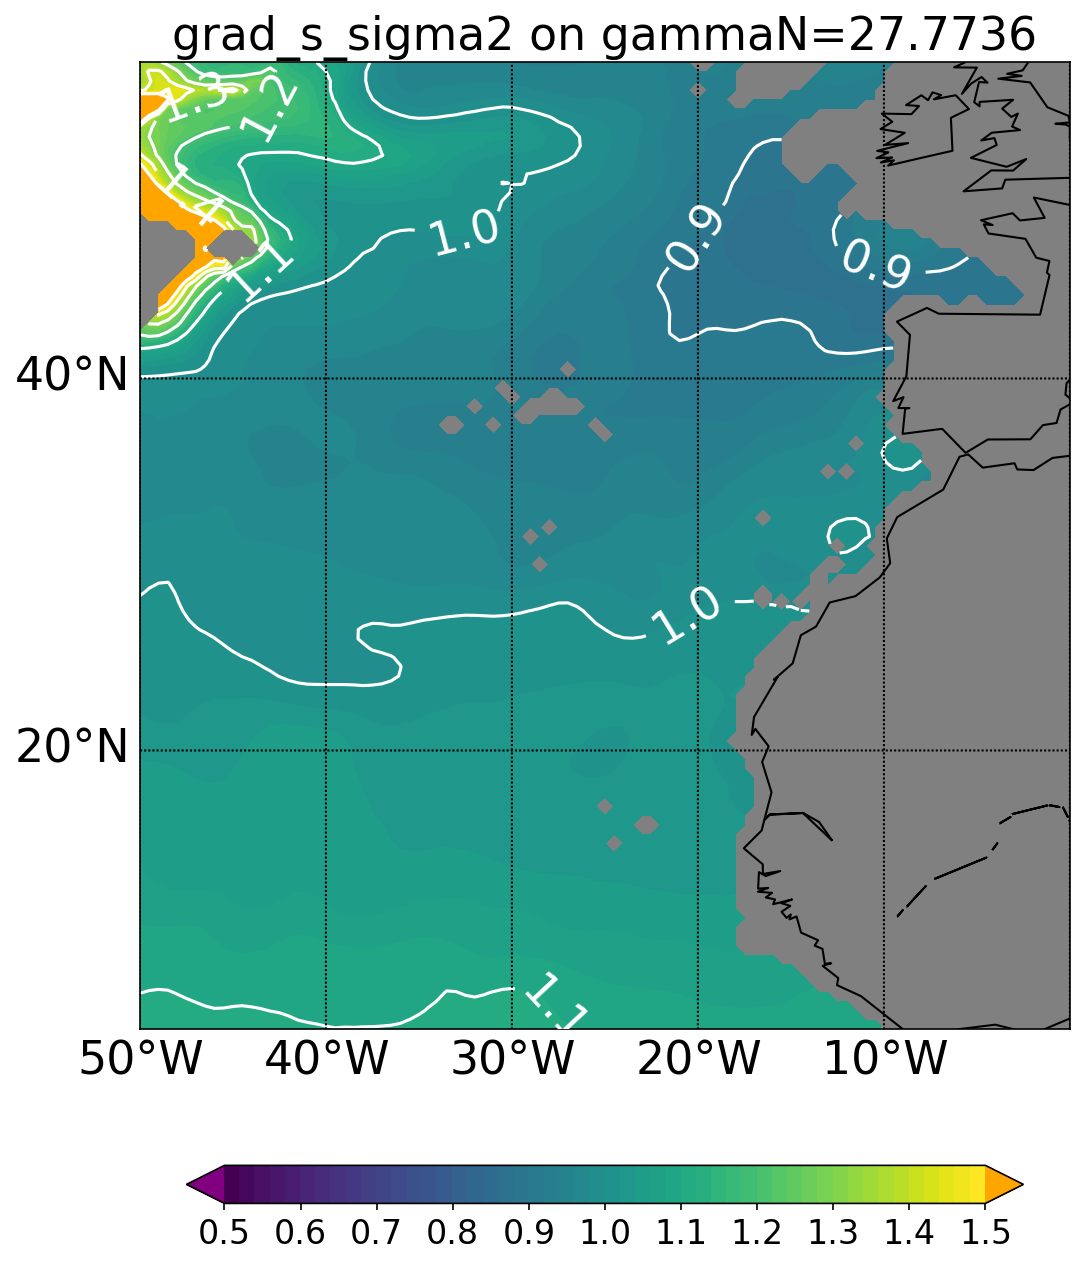
\includegraphics[width=\textwidth]{gradient_ratios/gibraltar_grad_s/Map2dcyl_grad_s_sigma2_on_gammaN_2777e-2_reg310Eto360E05Nto57N_1990to1998av_WOCE}
         \caption{Referenced to $p_{ref} = 2000$dbar}
         \label{fig:subplot_gibraltar_grad_s_sig2}
     \end{subfigure}
     
     \begin{subfigure}{0.4\textwidth}
         
         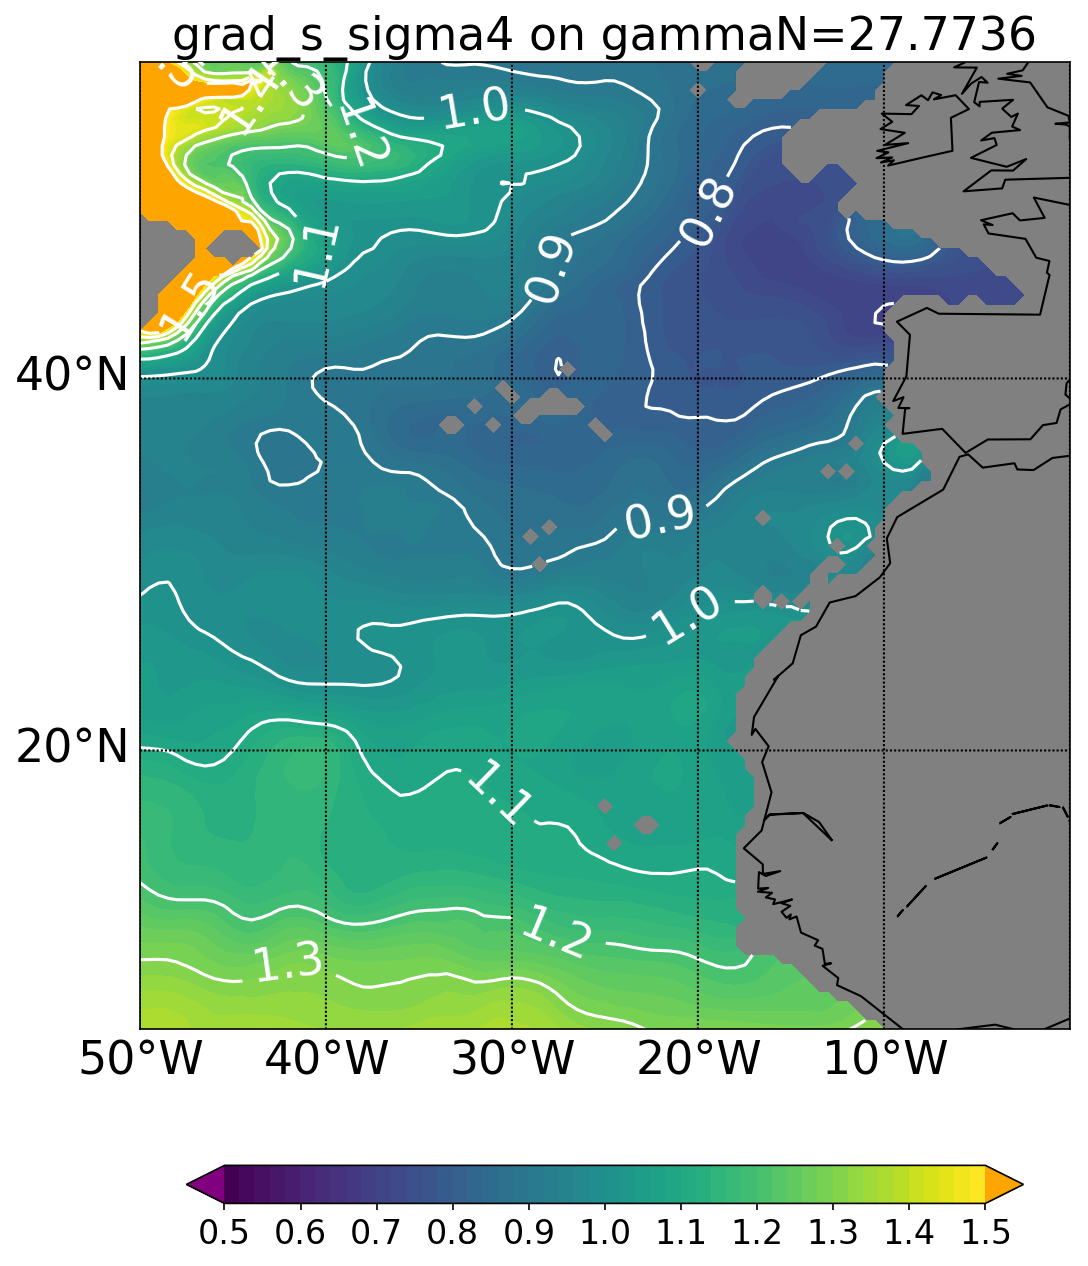
\includegraphics[width=\textwidth]{gradient_ratios/gibraltar_grad_s/Map2dcyl_grad_s_sigma4_on_gammaN_2777e-2_reg310Eto360E05Nto57N_1990to1998av_WOCE}
         \caption{Referenced to $p_{ref} = 4000$dbar}
         \label{fig:subplot_gibraltar_grad_s_sig4}
     \end{subfigure}
     
    \caption{Gradient ratio of $S$ for three reference pressures, 0, 2000 and 4000dbar which correspond to the $\sigma_0$, $\sigma_2$ and $\sigma_4$ potential density surfaces respectively, projected onto the neutral surface $\gamma_n = 27.7736$, Gibraltar region (see section \ref{subsubsection:spreadmethodgibraltarstraight})}
    \label{fig:gibraltar_grad_s}
    
\end{figure}

Figure \ref{fig:atlantic_grad_theta} shows that the gradient ratios of $\theta$ are reduced on the $\sigma_2$ and $\sigma_4$ surfaces, as we would expect. 

However, the $S$ gradient ratios seem to be split into two distinct regions. For reference pressures 2000dbar and 4000dbar below approximately $25^{\circ}$N the ratio is greater than one while above the majority is less than one. The regimes would be 2 and 3, respectively. The pattern is reversed for $p_{ref}=0$. 

In order to understand this we look at the values of $R_\rho$ and $c$ in the two regions. While the values of $c$ do not change much throughout the region the values of $R_\rho$ are highly variable. This result was also found in \citet{YOU2002}. 

For the Atlantic region it is clear from \ref{fig:subplot_atlantic_r_rho} that in general $R_\rho$ in the region is positive and greater than one, so the regime will not change. However, in the Gibraltar Straight we can see that there is a pattern that matches the regime change shown in the $S$ gradient ratio plots. Below $25^{\circ}$N $R_\rho$ is negative, placing surfaces $\sigma_2$ and $\sigma_4$ in regime 2, while above it is mainly positive and greater than one, placing those surfaces in regime 3. 

\begin{figure}[htbp]
    \centering
     \begin{subfigure}[b]{0.4\textwidth}
         
         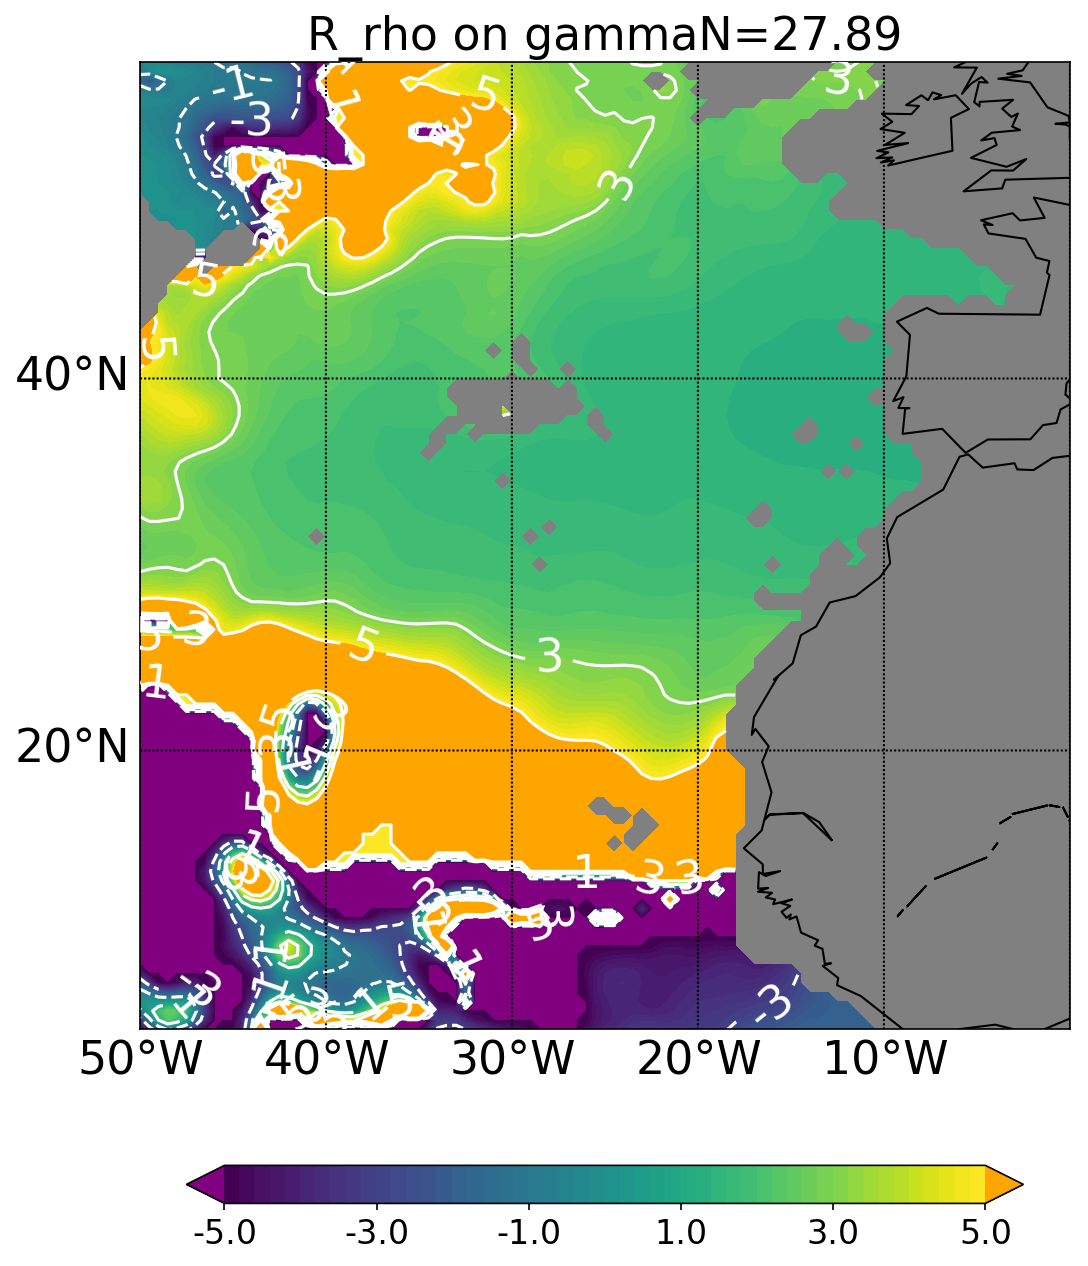
\includegraphics[width=\textwidth]{plots/R_rho/atlantic_r_rho/Map2dcyl_R_rho_on_gammaN_2789e-2_reg310Eto360E05Nto57N_1990to1998av_WOCE.png}
         \caption{$R_\rho$ on $\gamma_n = 27.89$, Atlantic}
         \label{fig:subplot_atlantic_r_rho}
     \end{subfigure}
     \hfill
     \begin{subfigure}[b]{0.4\textwidth}
         
         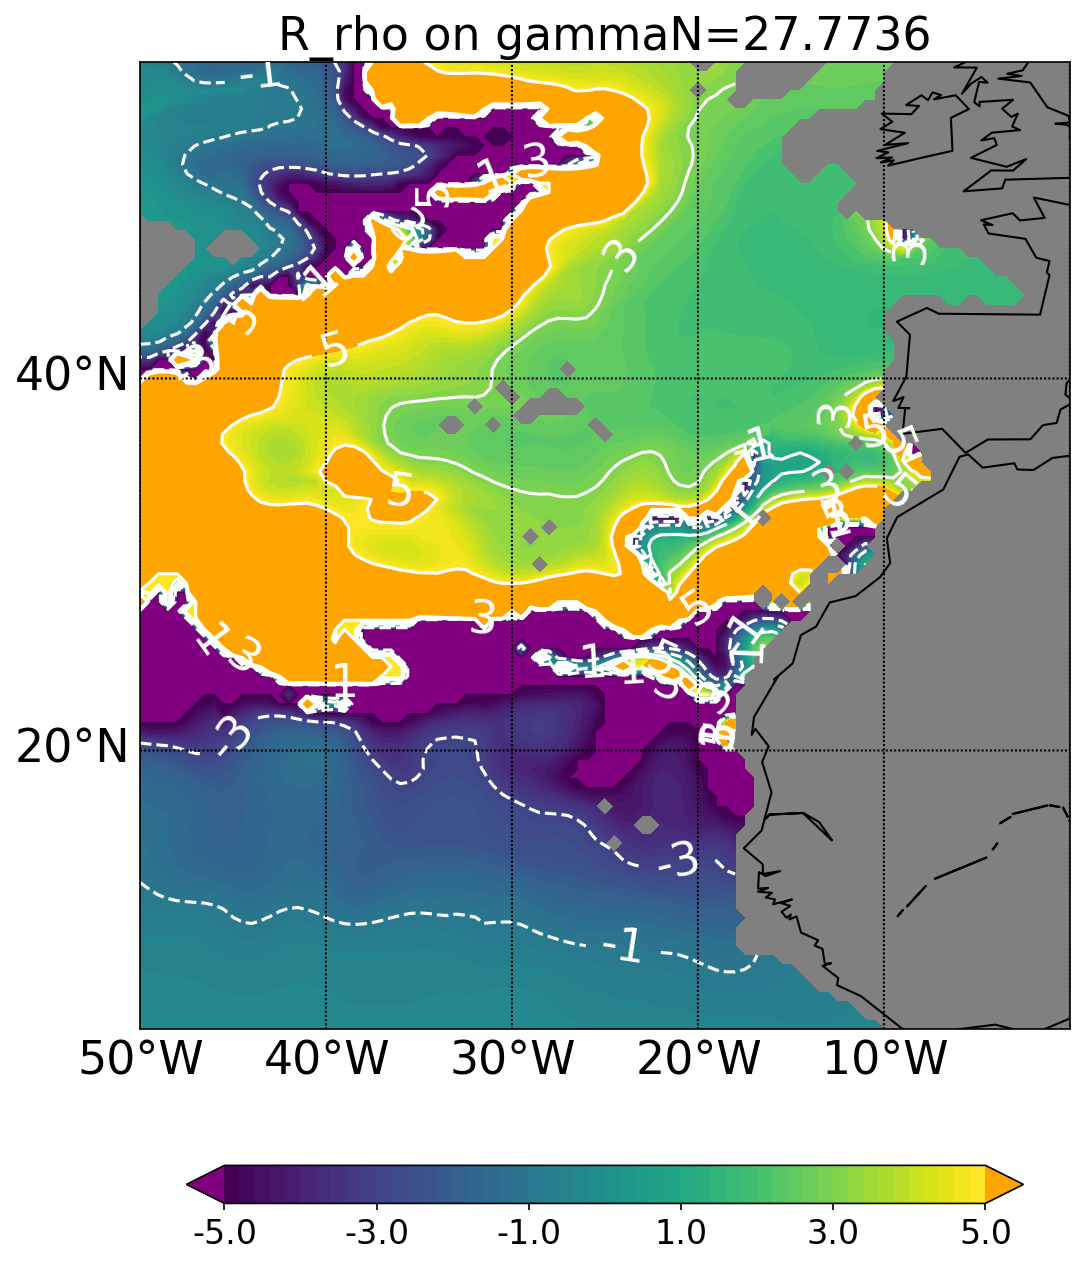
\includegraphics[width=\textwidth]{plots/R_rho/gibraltar_r_rho/Map2dcyl_R_rho_on_gammaN_2777e-2_reg310Eto360E05Nto57N_1990to1998av_WOCE.png}
         \caption{$R_\rho$ on $\gamma_n = 27.7736$, Gibraltar}
         \label{fig:subplot_gibraltar_r_rho}
     \end{subfigure}
     
    \caption{Density ratio $R_\rho$ projected onto the neutral surfaces $\gamma_n= 27.89$ for the Atlantic region and  $\gamma_n = 27.7736$ for the Gibraltar region (see section \ref{subsubsection:spreadmethodgibraltarstraight})}
    \label{fig:R_rho}
    
\end{figure}

This shows that the classification of surfaces into regimes is more complicated than might be expected: different parts of the same surface might lie in two or even three different regimes due to the high variance of $R_\rho$.